\documentclass[english,course]{lecture}

\usepackage{listings}
\usepackage{cleveref}
\usepackage{longtable}
\usepackage{tikz}
\usepackage{amsmath}
%--------------------------------------------------------------------------
% First, provide some data about this document
\title{lecture notes}
\subtitle{Cybersecurity Specialist}
%\shorttitle{Shortened title} % For headers; if undefined, the usual title will be used
\ccode{CS0424IT} % Most of these data are not compulsory
% \subject{Subject of the Talk}
\author{Simone La Porta}
% \spemail{speaker@email.com}
% \email{email@email.com}
% \speaker{Speaker's name}
\date{27}{05}{2024}
\dateend{13}{09}{2024}
% \conference{Lecture hall 7}
% \place{University of Physics}
\flag{\href{https://github.com/simone0509/CS0424IT}{
\includegraphics[scale=0.06]{images/github_logo.png}} \\ Written in \LaTeX}
% \attn{Place anything here to gather your readers' attention. This could be a warning, a disclaimer, a license, or, more likely, some helpful suggestions for your readers.}
% \morelink{https://github.com/simone0509/CS0424IT}
%-----------------------------------------------------------------------------


% And then begin your document
\begin{document}

\part{Unit 1: Fundamentals of Ethical Hacking}
\section{Introduction and Virtual Machines}\lecture[4 hours]{27}{05}{2024}

The Cybersecurity Specialist course aims to train professionals in the field of information security. These individuals will possess strong technical skills, providing added value to companies in the fight against cybercrime. The course is divided into three units:
\begin{enumerate}
    \item \textbf{Unit 1} focuses on the theoretical prerequisites and technical skills necessary for an Ethical Hacker. It covers topics such as networking, operating systems, and an introduction to programming;
    \item \textbf{Unit 2} centers on the phases of Penetration Testing, exploring the tools and techniques used by hackers in the real world;
    \item \textbf{Unit 3} provides students with a comprehensive understanding of how to monitor security events, manage ongoing attacks, and adopt best practices at the enterprise level to minimize the impact on business activities.
\end{enumerate}

In the past century, computing and the web were primarily the domain of experts, including hackers. The term \emph{hacker}, often associated with digital piracy, encompasses three distinct types of hackers:
\begin{itemize}
    \item \textbf{White Hat Hackers}, also known as "Ethical Hackers," operate with a strict adherence to ethical standards. Their work involves improving security with the consent of the system owner;
    \item \textbf{Grey Hat Hackers} operate in a legal and ethical gray area. They often act without the owner's permission but with the intent of improving security. While their actions can uncover vulnerabilities, they can also be controversial and sometimes illegal;
    \item \textbf{Black Hat Hackers} are criminals who break into computer networks with malicious intent. They may deploy malware to destroy files, steal information, hold computers hostage, or pilfer passwords, credit card numbers, and other personal data. Their motivations are typically opportunistic, such as financial gain. Stolen data is often sold on the dark web, where items like credit card details, online payment system access, medical records, and even streaming service accounts are traded.
\end{itemize}

An Ethical Hacker is a cybersecurity expert capable of simulating cyber-attacks to identify potential vulnerabilities in a company's systems. These simulations, known as \emph{Penetration Tests}, are crucial for detecting and fixing security issues in digital networks, software, and devices, thereby protecting enterprises and public entities from cybercriminal activities. Key responsibilities of an Ethical Hacker include:
\begin{itemize}
    \item Conducting penetration tests on IT infrastructures and web applications;
    \item Ensuring the security of sensitive and private data, such as payment details, login credentials, and passwords.
\end{itemize}

It is crucial to emphasize that penetration testing should only be performed with the formal consent of the system or network owner. Conducting such tests without permission is illegal and can lead to severe legal consequences.


\subsection{Virtualization Process}
Virtual machines (VMs) are emulations of computer systems that provide the functionality of a physical computer. They run on a physical host machine and are managed by a virtualization layer. The process of creating and managing VMs is known as virtualization (\Cref{fig:virtualization}).
Virtualization involves several key steps:

\begin{enumerate}
    \item \textbf{Hypervisor Installation:} The hypervisor, also known as the Virtual Machine Monitor (VMM), is installed on the host machine. The hypervisor can be of two types:
    \begin{itemize}
        \item \textbf{Type 1 (Bare Metal):} Runs directly on the host's hardware.
        \item \textbf{Type 2 (Hosted):} Runs on top of an existing operating system.
    \end{itemize}
    \item \textbf{Resource Allocation:} The hypervisor allocates resources (CPU, memory, storage, and network) from the physical host to each VM.
    \item \textbf{VM Creation:} Virtual machines are created by defining their virtual hardware specifications (number of CPUs, amount of memory, disk size, etc.).
    \item \textbf{Operating System Installation:} An operating system is installed on the virtual machine, just as it would be on a physical machine.
    \item \textbf{VM Management:} The hypervisor manages the execution of VMs, handles resource allocation dynamically, and ensures isolation between VMs.
\end{enumerate}

\begin{figure}
    \begin{center}
        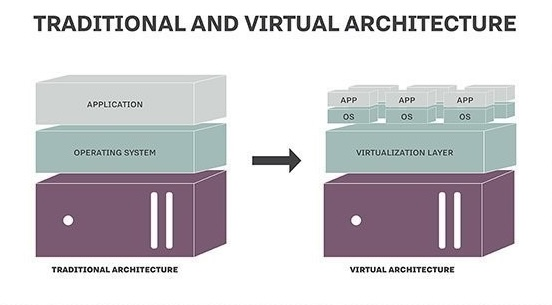
\includegraphics[width=\textwidth]{images/virtualization.jpg}
        \caption{Traditional vs Virtual architecture.}
        \label{fig:virtualization}
    \end{center}
\end{figure}


\subsubsection{Virtual Hardware}
A virtual machine emulates physical hardware components such as:
\begin{itemize}
    \item \textbf{CPU:} Virtual CPUs (vCPUs) are assigned to the VM by the hypervisor.
    \item \textbf{Memory:} Virtual memory is allocated from the host's physical memory.
    \item \textbf{Storage:} Virtual disks are created using files on the host's storage system.
    \item \textbf{Network:} Virtual network interfaces connect VMs to the host's network and to other VMs.
\end{itemize}

\subsubsection{Hypervisor Role}
The hypervisor plays a critical role in:
\begin{itemize}
    \item \textbf{Resource Management:} Dynamically allocating resources to VMs based on their needs.
    \item \textbf{Isolation:} Ensuring that each VM operates independently and securely.
    \item \textbf{Efficiency:} Optimizing resource usage to maximize the performance of VMs.
\end{itemize}

\subsubsection{Execution Flow}
The execution flow of a VM includes:
\begin{enumerate}
    \item \textbf{Boot Process:} The VM goes through a boot process similar to a physical machine, loading its operating system from the virtual disk.
    \item \textbf{Application Execution:} Applications run within the VM, utilizing the virtualized hardware.
    \item \textbf{Hypervisor Interaction:} The VM interacts with the hypervisor for tasks like I/O operations, which the hypervisor translates to the physical hardware.
\end{enumerate}

\subsubsection{Benefits of Virtualization}
Virtualization offers several advantages:
\begin{itemize}
    \item \textbf{Cost Efficiency:} Reduces the need for physical hardware.
    \item \textbf{Scalability:} Easily create, modify, and delete VMs as needed.
    \item \textbf{Isolation:} Provides a secure and isolated environment for each VM.
    \item \textbf{Resource Utilization:} Maximizes the usage of physical resources.
\end{itemize}

Virtualization is a powerful technology that enables the efficient use of hardware resources, providing flexibility, scalability, and isolation. Virtual machines are an integral part of modern computing environments, supporting a wide range of applications from development to production systems.

\section{Networking}\lecture[4 hours]{28}{05}{2024}\lecture[4 hours]{29}{05}{2024}
\subsection{Network Categories: Geographical and Topological}
\subsubsection{Geographical Networks}

Networks can be categorized based on the geographical distance between devices. The primary types of geographical networks include:

\paragraph{WAN - Wide Area Network}
Wide Area Networks (WANs) connect computers over large distances, covering extensive geographical areas. WANs use various transmission methods such as satellites, fiber optics, and cables. The quintessential example of a WAN is the Internet, which allows computers in different continents to communicate within seconds.

\paragraph{LAN - Local Area Network}
Local Area Networks (LANs) connect computers within a smaller geographical area, such as the floors of a building in a company. LANs are popular due to their high speed and relative ease of installation.

\paragraph{PAN - Personal Area Network}
Personal Area Networks (PANs) cover very limited areas, such as the connection between a mobile phone and a computer.

\subsubsection{Topological Networks}

Networks can also be categorized based on their physical configuration. The primary types of topological networks include the following, also shown in \Cref{fig:net_topo}.

\begin{figure}[h]
    \centering
    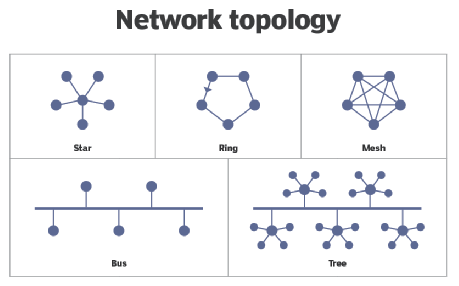
\includegraphics[width=\textwidth]{images/network_topology.png}
    \caption{Network topologies.}
    \label{fig:net_topo}
\end{figure}

\paragraph{Bus Topology}
In a bus topology, devices share a single transmission channel, typically a single cable. One of the advantages of bus topology is its simplicity and ease of implementation.

\paragraph{Ring Topology}
In a ring topology, devices are connected in a circular manner. These networks are more complex and expensive than bus networks and are generally used in enterprise environments for corporate LANs.

\paragraph{Star Topology}
In a star topology, devices are individually connected to a central device, such as a switch or router, using dedicated cables or other physical media. Each computer has a dedicated link to the central device and can communicate with other devices through it. Star networks are the most widely used due to their performance and security characteristics.

Understanding the different types of networks, both geographical and topological, is essential for designing and implementing efficient and secure network infrastructures. WANs, LANs, and PANs cater to different geographical scopes, while bus, ring, and star topologies offer various configurations to meet specific organizational needs.


\subsection{Basic Networking Concepts}

A computer network enables and facilitates communication between people, applications, and servers regardless of their geographical location. The Internet is the largest example of a computer network that we use on a daily basis. In a computer network, machines communicate with each other using communication \textit{protocols}, which ensure communication between computers with different hardware and software.

\subsubsection{Data Transmission}

Communication occurs through an exchange of data, or information, which is transported in the form of \textit{packets}. Packets are streams of bits exchanged via electrical signals over a physical medium. The physical medium can be a LAN (local area network) cable or, very commonly, the air in a Wi-Fi network.

\begin{figure}[h]
    \centering
    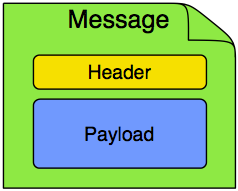
\includegraphics[width=0.4\textwidth]{images/message.png}
    \caption{Structure of a Packet: Header and Payload.}
    \label{fig:packet_structure}
\end{figure}

\subsubsection{Packet Structure}

A \textit{packet} has a defined structure as shown in \Cref{fig:packet_structure}. The \textit{Header} depends on the protocol used in the communication. Its task is to ensure that the receiving computer can interpret the \textit{Payload} and manage the communication. The \textit{Payload}, on the other hand, is the actual information. For instance, it could be a message, or part of a message sent from one computer to another, an email, or other data.

\subsection{The ISO/OSI Model}

To standardize network communication, in 1984 the International Organization for Standardization (ISO) published a theoretical model subsequently called the \textit{Open System Interconnection (OSI)} model. The ISO/OSI model is used as a theoretical reference. It is based on a stack of 7 layers, also called \textit{layers}, where each layer serves the upper layer and has exclusive protocols.

\begin{figure}[h]
    \centering
    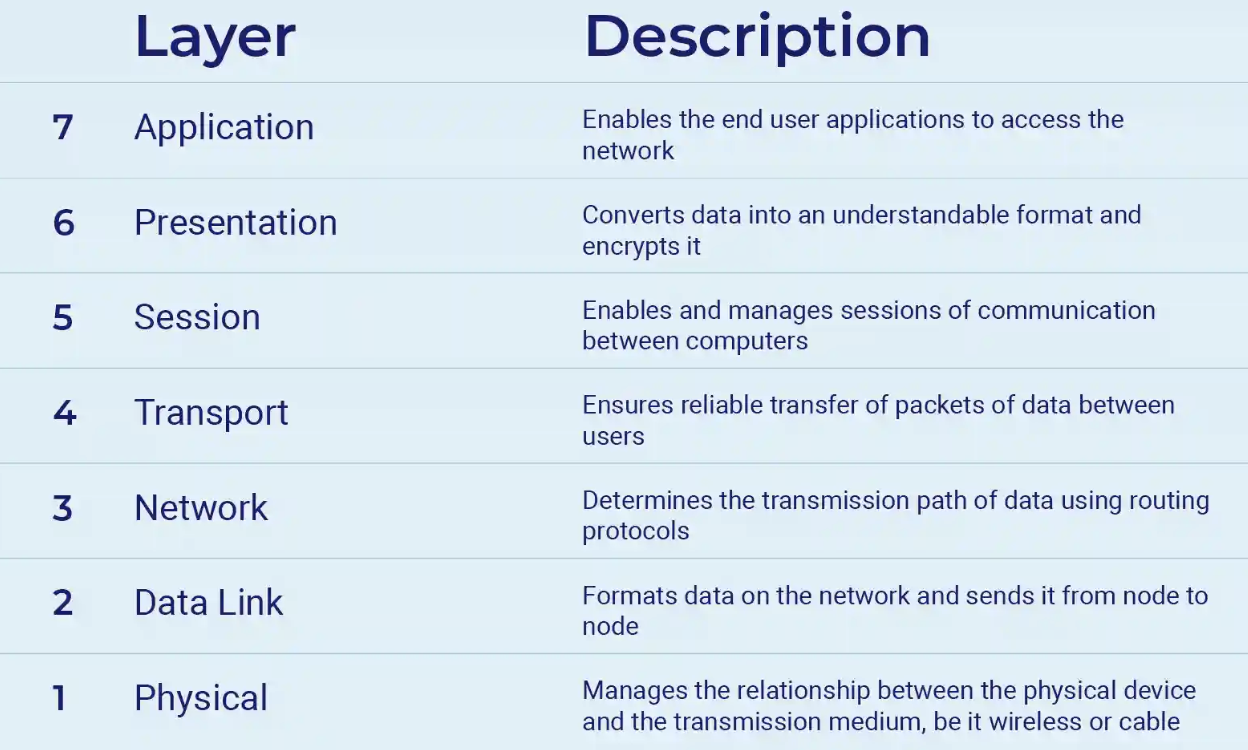
\includegraphics[width=\textwidth]{images/layers_osi.png}
    \caption{The ISO/OSI Model Layers.}
    \label{fig:osi_layers}
\end{figure}

In a communication between two computers, the data follows the logical model as represented by the line in \Cref{fig:osi_model}.

\begin{figure}[h!]
    \centering
    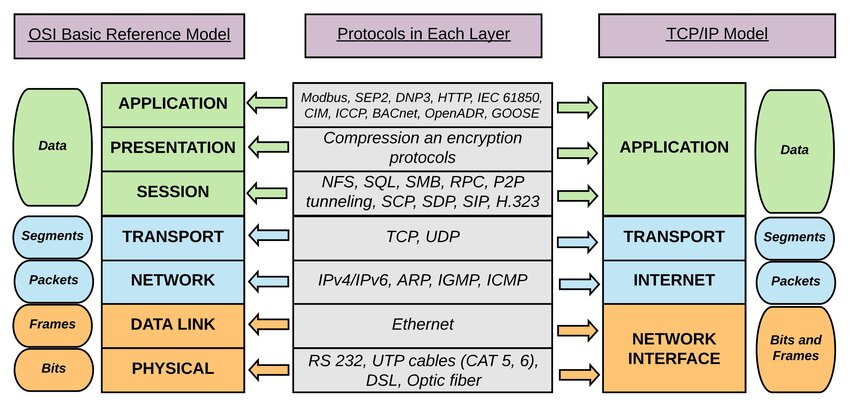
\includegraphics[width=\textwidth]{images/iso_osi_tcp.png}
    \caption{The ISO/OSI vs TCP/IP model.}
    \label{fig:osi_model}
\end{figure}

Note that the ISO/OSI model is a theoretical model to be used as a reference. In practice, applications use the \textit{TCP/IP} model, which slightly varies from the theoretical ISO/OSI model.

The differences between TCP/IP and the ISO/OSI model are depicted in \Cref{fig:osi_model} and summarized in \Cref{fig:tcp_vs_osi}. For theoretical study of concepts, we will follow the notions of the ISO/OSI model.

\begin{figure}[h!]
    \centering
    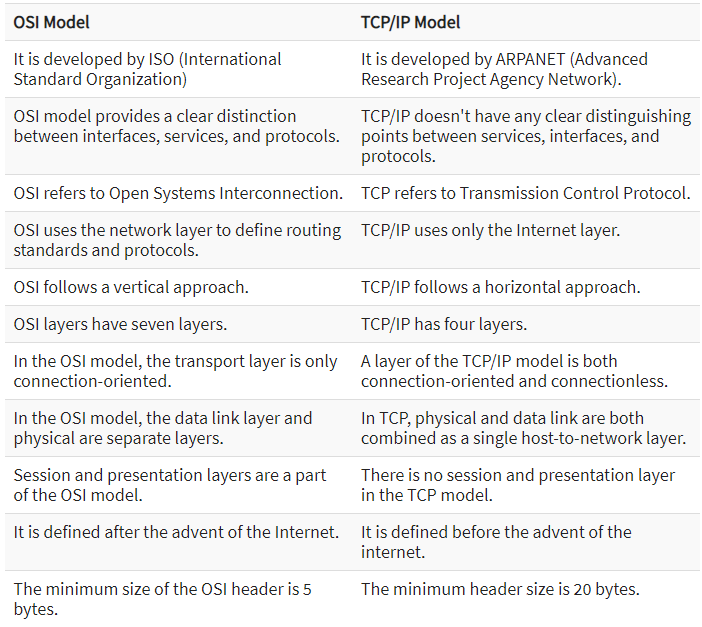
\includegraphics[width=\textwidth]{images/tcp_vs_osi.png}
    \caption{The ISO/OSI vs TCP/IP model.}
    \label{fig:tcp_vs_osi}
\end{figure}


\subsubsection{\textbf{Physical Layer}}
The physical layer is responsible for the transmission of raw data bits over a physical medium. This transmission can occur via various types of cabling, such as copper wires or fiber optics. Data from higher layers of the source computer is segmented and sent to the physical layer of the receiving computer in the form of bits.

\paragraph{Bits and Binary System}
The bit, short for binary digit, is the basic unit of information in computing, represented as either '0' or '1'. Unlike the decimal system, which uses ten digits (0-9), computers operate using the binary system. Consequently, information is transmitted over a physical cable as a sequence of binary digits, for example, 10010010 10011110, etc.

\subsubsection{\textbf{Data Link Layer}}
The Data Link Layer utilizes the services of the physical layer to send and receive bits over communication channels. Packets at this layer are referred to as frames. The main functions of the Data Link Layer include:

\begin{itemize}
    \item Providing an interface to the Network Layer (Layer 3)
    \item Handling transmission errors
    \item Regulating the flow of bits between two communicating devices
\end{itemize}

The Data Link Layer plays a crucial role by defining protocol standards such as IEEE 802.3 for Ethernet (wired connections) and IEEE 802.11 for Wireless connections.

\paragraph{MAC Address}
In a computer network, two personal computers communicate at the Data Link Layer using what is called a physical address or more commonly, a MAC Address. The MAC address is a 48-bit identifier typically represented in hexadecimal format. Below is a table showing the conversion between binary and hexadecimal systems:

\begin{table}[h]
    \centering
    \begin{tabular}{|c|c|}
        \hline
        \textbf{Binary} & \textbf{Hexadecimal} \\
        \hline
        0000 & 0 \\
        0001 & 1 \\
        0010 & 2 \\
        0011 & 3 \\
        0100 & 4 \\
        0101 & 5 \\
        0110 & 6 \\
        0111 & 7 \\
        1000 & 8 \\
        1001 & 9 \\
        1010 & A \\
        1011 & B \\
        1100 & C \\
        1101 & D \\
        1110 & E \\
        1111 & F \\
        \hline
    \end{tabular}
    \caption{Binary to Hexadecimal Conversion}
    \label{tab:bin_hex}
\end{table}

An example of a MAC Address is 00:AA:11:BB:22:CC. The MAC address is a unique identifier assigned to the network interfaces of devices.

\paragraph{Ethernet Frame Structure}
The structure of an Ethernet 802.3 frame includes fields for the Destination MAC Address and the Source MAC Address. These fields are automatically populated with the MAC addresses of the source and destination when an exchange of information begins at the Data Link Layer.

\paragraph{Role of Switches}
Switches are vital network devices for communication but come with certain disadvantages. They route broadcast packets across the entire network. Broadcast packets are sent to a specific MAC address, FF:FF:FF:FF:FF:FF, which is received by the switch and routed to all nodes connected to it. This creates what is known as a broadcast domain.

A broadcast domain includes all the devices on a network segment that receive broadcast frames from any device within the segment. In a large network with numerous devices, this can cause significant latency issues.

\paragraph{Address Resolution Protocol (ARP)}
ARP, or Address Resolution Protocol, is a network protocol used to map IP addresses to MAC addresses within a local network. Its primary functions include:

\begin{itemize}
    \item \textbf{ARP Request}: A device broadcasts an ARP request on the local network, asking for the MAC address associated with a specific IP address.
    \item \textbf{ARP Reply}: The destination device responds with a packet containing its MAC address associated with the requested IP address.
    \item \textbf{ARP Cache}: Devices maintain an ARP table or ARP cache that stores IP-to-MAC address mappings.
\end{itemize}


ARP is crucial for communication within the same local network. When a device needs to send data to another device within the same subnet, it uses ARP to discover the MAC address corresponding to the destination IP address.

\paragraph{Virtual LAN (VLAN)}\lecture[4 hours]{30}{05}{2024}
Switches allow the segmentation of broadcast domains through the creation of Virtual LANs (VLANs). A VLAN is a logical grouping of hosts and network devices. VLANs are created by adding a "tag" or VLAN ID to the switch ports, or by mapping the MAC address of the host to the VLAN ID.

Assume we want to restrict communication and the broadcast domain to hosts A, B, and C. We create a VLAN identified by ID 100 and associate the MAC addresses of hosts A, B, and C with that VLAN.

When host A sends a packet to the broadcast address, it will only be received by hosts B and C. Therefore, VLANs segment broadcast domains and eliminate latency issues in large networks.


VLANs are essential for managing broadcast domains within a network. By associating specific MAC addresses with VLAN IDs, we can ensure that broadcast traffic is limited to only those hosts within the same VLAN, thus improving network efficiency and reducing latency.


\subsubsection{\textbf{Network Layer}}
In networking, just as there are specific devices at the Data Link Layer that facilitate communication between personal computers on the same network, there are devices at the Network Layer, such as router-gateways, that enable data routing between personal computers connected to different networks. For instance, consider the following network configuration:

\paragraph{Role of the Router}
A switch operates at Layer 2 and does not route packets to other networks because it forwards packets based on MAC addresses rather than IP addresses. The solution is to use a Layer 3 device like a router-gateway.

The router receives the packet from the switch and checks its routing table to determine which of its interfaces to forward the packet to reach the destination network.

\paragraph{Example of Router Operation}
To better understand how a router-gateway functions, consider a router connected with three interfaces to three different networks:

If a personal computer on network $2.228.1.0$ wants to send a packet to a PC on network $2.175.1.0$, the packet will be sent to the router, which will check its routing table to see which interface to use to forward the packet.

In a network, computers interact using both MAC and IP addresses. For example, if PC A wants to send a packet to PC B, it will structure the packet as follows:

\begin{itemize}
    \item The destination IP address of B in the datagram header (Layer 3).
    \item The MAC address of the router as the destination in the frame header (Layer 2). The router, in this case, is the "next hop."
    \item Its IP address as the source in the datagram header.
    \item Its MAC address as the source in the frame header.
\end{itemize}

The router will receive the packet and set:
\begin{itemize}
    \item The destination MAC address to that of B.
    \item The source MAC address to that of its corresponding interface.
\end{itemize}

Routers play a crucial role in network communication by enabling the routing of data between different subnets. This process involves intricate interactions between Layer 2 (MAC addresses) and Layer 3 (IP addresses) addressing schemes, ensuring seamless communication across diverse network segments.

\subsubsection{\textbf{Transport Layer}}
The transport layer, also known as layer 4 in the OSI model, is responsible for establishing a logical connection or channel between applications on different computers. It ensures the reliable transmission of data packets between a source and a destination. Packets may get lost during transmission due to network congestion, communication errors, or network issues. In some scenarios, minor transmission issues are tolerable, such as in phone conversations or video streaming, where a lost packet might result in a brief glitch. However, for activities like financial transactions or logging into a portal, it's crucial that communication is lossless.

\paragraph{Protocols in the Transport Layer}
The transport layer provides two fundamental protocols for communication between hosts:
\begin{itemize}
    \item \textbf{TCP (Transmission Control Protocol)}: TCP guarantees data traffic control and reliable delivery to the recipient, making it more secure for applications requiring guaranteed packet delivery. The reliability of TCP is due to its connection-oriented nature, which establishes a communication channel before data exchange. TCP follows a three-step process called the \textit{three-way handshake} to establish this connection.
    \begin{enumerate}
        \item The client initiating the connection sends a TCP packet with the SYN flag set and a random sequence number.
        \item The server responds with a packet that has both SYN and ACK flags set, along with its own sequence number and an acknowledgment number equal to the client's sequence number plus one.
        \item The client completes the synchronization by sending a packet with the ACK flag set, acknowledging the server's sequence number.
    \end{enumerate}
    \item \textbf{UDP (User Datagram Protocol)}: UDP is a connectionless protocol that does not require establishing a communication channel before data exchange. It is more lightweight and faster, suitable for activities requiring data streaming (e.g., video or audio). However, it does not guarantee packet delivery.
\end{itemize}


\paragraph{Ports and Services}
To identify the target process or service for a given packet, both TCP and UDP use ports, represented as \texttt{<ip>:<port>}. While the IP identifies the destination machine, the port provides information about the service. Ports can be categorized into:

\begin{itemize}
    \item \textbf{Well-known ports}: Used for standard services, ranging from 0 to 1023.
    \item \textbf{High ports}: Used for non-standard services, ranging from 1024 to 65535.
\end{itemize}

\begin{table}[h]
    \centering
    \begin{tabular}{|c|c|}
        \hline
        \textbf{Protocol} & \textbf{Port} \\
        \hline
        SMTP & 25 \\
        SFTP & 115 \\
        HTTP & 80 \\
        HTTPS & 443 \\
        SSH & 22 \\
        Telnet & 23 \\
        POP3 & 110 \\
        FTP & 21 \\
        \hline
    \end{tabular}
    \caption{Commonly Used Ports}
    \label{tab:ports}
\end{table}

Understanding the transport layer is crucial for ensuring reliable communication between applications on different hosts. TCP and UDP provide different levels of service, making them suitable for various applications. TCP's connection-oriented nature and reliable delivery make it ideal for critical applications, while UDP's connectionless nature and speed make it suitable for real-time data streaming.


\subsubsection{\textbf{Session Layer}}
In order to enable communication between two hosts, or between a client and a server, it is necessary to first establish a session. This is precisely the role of the protocols that are part of the session layer. Sessions are essential to ensure the correct transfer of information. It is very important to define the rules for opening, closing, or maintaining a session. We can identify two main purposes of the session layer:

\begin{itemize}
    \item Definition and management of the session:
    \begin{itemize}
        \item \textbf{Initiating or opening a session} between a user who intends to use a service that is listening on a specific server. A common example is the \textit{SSH} (Secure Shell) protocol, which is used by system administrators to create sessions on remote servers.
        \item \textbf{Maintaining the session} for its duration, ensuring the session remains active during the flow of information.
        \item \textbf{Closing the session}, either upon the request of the user or the server.
    \end{itemize}
    \item Synchronization: saving intermediate checkpoints (or synchronization points) during a data flow. This allows for the preservation of information in the event of an abnormal session interruption.
\end{itemize}

\subsubsection{\textbf{Presentation Layer}}
The Presentation Layer is the sixth level in the OSI (Open Systems Interconnection) model. This layer is responsible for the preparation of data in transit between two hosts before it is presented to the users. One of the critical functions of the Presentation Layer is \textbf{data encryption}. In a communication channel, data can transit in one of two ways:

\begin{itemize}
    \item \textbf{In clear text}: Data is transmitted in a visible and readable form to everyone.
    \item \textbf{Encrypted}: Data is encoded such that only authorized parties can view the content.
\end{itemize}

Encryption transforms clear text data into encrypted data using what is known as an \textbf{encryption algorithm}. The primary purpose of encryption is to ensure that the content of the information is available only to specific users, thereby securing the data from potential malicious actors.

The Presentation Layer performs several critical functions, including:

\begin{enumerate}
    \item \textbf{Translation}: This layer translates data between the application layer and the network format. It ensures that data from the sender's application layer can be understood by the receiver's application layer.
    \item \textbf{Data Encryption and Decryption}: As mentioned, encryption is a fundamental aspect of the Presentation Layer. It encodes the data before it is transmitted over the network and decodes it upon arrival.
    \item \textbf{Data Compression}: The Presentation Layer can compress data to reduce the bandwidth needed for transmission. This can lead to faster transmission times and reduced network load.
    \item \textbf{Character Code Translation}: It translates character codes from one coding system to another. For example, it can convert ASCII to EBCDIC.
    \item \textbf{Data Serialization}: This process involves converting complex data structures into a format that can be easily transmitted over the network.
\end{enumerate}

\paragraph{Encryption}
Encryption is a process that involves transforming readable data, known as \textbf{plaintext}, into an unreadable format, known as \textbf{ciphertext}. This transformation uses an algorithm and an encryption key. Only authorized parties who possess the corresponding decryption key can convert the ciphertext back into readable plaintext.

Encryption serves several essential purposes:

\begin{itemize}
    \item \textbf{Confidentiality}: Ensures that data is only accessible to those who have the appropriate decryption key.
    \item \textbf{Integrity}: Protects data from being altered during transmission.
    \item \textbf{Authentication}: Verifies the identities of the communicating parties.
    \item \textbf{Non-repudiation}: Prevents parties from denying the transmission or receipt of data.
\end{itemize}

The Presentation Layer plays a crucial role in ensuring that data is properly encrypted and decrypted, thereby maintaining the security and integrity of the information being transmitted across networks.


\subsubsection{\textbf{Application Layer}}
The application layer is the seventh and final layer of the ISO/OSI model. This layer interacts directly with the applications used by the end user, providing interface services for applications and support for network access. Among the most well-known protocols of the application layer are:

\begin{itemize}
    \item \textbf{HTTP/HTTPS (Hyper Text Transfer Protocol):} This is the main protocol for transmitting information on the web. HTTPS is the secure, encrypted version of HTTP. The protocol operates on a request/response mechanism, typical of the client/server model, where a host requests a resource from a remote web server.

    \item \textbf{DNS (Domain Name System):} This protocol translates domain name requests (e.g., \texttt{www.google.com}) into IP addresses. DNS is a fundamental protocol for the functioning of the internet. A DNS name like \texttt{www.store.google.com} can be divided as follows:
    \begin{itemize}
        \item \texttt{www} - Host
        \item \texttt{store} - Subdomain
        \item \texttt{google} - Domain
        \item \texttt{com} - Top-Level Domain (TLD)
    \end{itemize}
    The resolution of DNS names is handled by DNS resolvers, which are DNS servers generally provided by ISPs (Internet Service Providers), such as Vodafone, TIM, or Wind3. Public DNS servers, like Google's DNS, are also available.

    \item \textbf{FTP (File Transfer Protocol):} This protocol manages the transfer of data between hosts and is based on TCP.

    \item \textbf{DHCP (Dynamic Host Configuration Protocol):} This protocol allows devices on a LAN to receive network configuration automatically. An host connecting to a network where the DHCP service is active will have its IP address and other network information auto-assigned. For example, when you connect to your home network, you likely don't manually assign an IP address to your PC or smartphone. This is because DHCP is typically enabled on private networks for automatic IP assignment.
\end{itemize}

The application layer provides crucial functionalities that directly support user applications and network services. Here are some key points:

\begin{itemize}
    \item \textbf{User Interface Support:} This layer offers services that directly interface with user applications, enabling seamless communication and data transfer over the network.

    \item \textbf{Protocol Implementation:} Protocols at this layer define the rules for communication between different devices and software applications. These protocols include not only HTTP, DNS, FTP, and DHCP but also others like SMTP (Simple Mail Transfer Protocol), POP3 (Post Office Protocol), and IMAP (Internet Message Access Protocol), which are used for email transmission and retrieval.

    \item \textbf{Resource Sharing:} It facilitates resource sharing across the network, such as file transfers, web pages, and email.

    \item \textbf{Network Transparency:} It provides a way for applications to interact with the network in a manner that abstracts the complexities of lower-layer operations, making network interactions more user-friendly and efficient.
\end{itemize}

The application layer is indispensable for ensuring that user applications can operate over the network effectively, providing the necessary protocols and services to support diverse network-based activities.


\subsection{Network Address Translation (NAT)}
Network Address Translation (NAT) is a technology developed to address the exhaustion of IPv4 addresses. Introduced in the 1990s, it delineates the distinction between private and public IP addresses. NAT is typically configured on routers or firewalls.

A public IP address allows devices to access the Internet, whereas private IP addresses are used within local networks (e.g., home or corporate networks) and are not directly accessible from the Internet. There are various types of NAT, but the basic concept involves translating private IP addresses (used within the local network) into one or more public IP addresses.

\subsection{Port Address Translation (PAT)}
Port Address Translation (PAT) is a specific form of NAT. In addition to translating IP addresses, PAT also translates the port numbers of devices within the local network. Ports are 16-bit numbers associated with each connection, and PAT enables multiple devices to share the same public IP address by distinguishing their connections based on port numbers.

For instance, if you have three devices using PAT and sharing the same public IP address, the first device's connection might use port 5000, the second device might use port 5001, and the third device might use port 5002. This allows the router to keep track of which connection belongs to which device on the local network.

In summary, while NAT translates private IP addresses into one or more public IP addresses, PAT goes further by also translating ports. This enables multiple devices to share the same public IP address, distinguishing them based on the ports used. Both technologies are fundamental for managing the scarcity of public IP addresses and enabling Internet connectivity for multiple devices within a local network.

\paragraph{Private IP Address Ranges}
The following table lists the ranges of IP addresses defined as "private." These IP addresses are assigned only within private networks and are not exposed or reachable via the Internet.

\begin{figure}[h!]
    \centering
    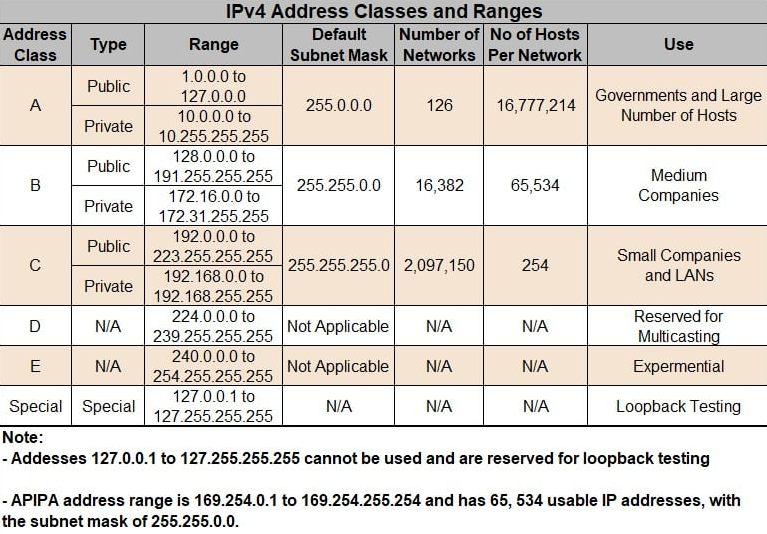
\includegraphics[width=0.8\textwidth]{images/ip_addresses.png}
    \caption{IP addresses types.}
    \label{fig:ip_address}
\end{figure}

\section{Operating Systems \& Programming Languages}
\lecture[4 hours]{03}{06}{2024}
A firewall is a crucial component in the realm of cybersecurity. It acts as a barrier that protects a network or system from external threats by managing and filtering incoming and outgoing network traffic. Essentially, a firewall serves as a gatekeeper between an internal network and the broader internet, analyzing network traffic and determining whether to allow or block data packets based on pre-established security rules.



\subsection{Key Classifications of Firewalls}

\begin{enumerate}
    \item \textbf{Firewall Types by Implementation:}
    \begin{itemize}
        \item \textbf{Hardware Firewalls:} These are physical devices dedicated to the task of network security. They are typically used by businesses and organizations with significant network traffic and complex security needs.

        \emph{Advantages}: high performance due to dedicated resources, capable of handling large volumes of traffic, centralized security management.

        \emph{Disadvantages}: higher cost and maintenance ,complexity in configuration and deployment.

        \item \textbf{Software Firewalls:} These are programs installed on individual computers or servers. They provide a flexible and often more economical solution, especially for personal use or smaller networks.

        \emph{Advantages}: cost-effective and easy to install, flexible and can be customized for specific needs, useful for personal devices and small businesses.

        \emph{Disadvantages}: consumes system resources, which can affect performance, requires individual management on each device.
    \end{itemize}

    \item \textbf{Firewall Placement:}
    \begin{itemize}
        \item \textbf{Perimeter Firewalls:} Positioned at the boundary of a network, perimeter firewalls are designed to safeguard the internal network from external threats. They act as the first line of defense, regulating access between the internal network and the internet or other untrusted networks.

        \emph{Advantages}: provides a robust first line of defense, centralized point of security control for the entire network.

        \emph{Disadvantages}: cannot protect against threats that bypass the perimeter, such as internal attacks.


        \item \textbf{Host-based Firewalls:} These are installed on individual devices within the network. They monitor and control traffic to and from the device on which they are installed, providing an additional layer of security.

        \emph{Advantages}: adds an extra layer of protection for individual devices, useful for controlling local traffic and internal threats.

        \emph{Disadvantages}: requires installation and management on each individual device, potentially increases the complexity of the overall security infrastructure.
    \end{itemize}
\end{enumerate}

\subsection{Types of traffic filtering}
Firewalls implement various types of traffic filtering to control which data packets can pass through or be blocked. Each type of firewall and filtering mechanism offers different levels of security and control over the network traffic.

\subsubsection{Static Packet Filtering}
Static packet filtering is a type of network traffic filtering where decisions to permit or block traffic are based on static criteria, such as IP addresses, source and destination ports, and protocols.

\begin{itemize}
    \item \textbf{Static Rules}: The firewall is configured with static rules created by the network administrator. These rules specify the criteria based on which the firewall evaluates the traffic.
    \item \textbf{Traffic Evaluation}: When the firewall receives a data packet, it compares the packet against the static rules. For example, it can check if the source and destination IP addresses are allowed, if the destination port is authorized, and if the protocol used is permitted.
    \item \textbf{Blocking or Permitting Decisions}: Based on these static rules, the firewall decides whether to permit or block the packet. If the packet matches the specified rules, it is allowed through; otherwise, it is blocked.
\end{itemize}

\subsubsection{Stateful Filtering}
Stateful filtering is an advanced type of filtering. Its distinguishing feature is the ability to track the state of network connections, enabling the firewall to make decisions based on contextual information about the connection.

\begin{itemize}
    \item \textbf{Initiated Connections}: A stateful firewall keeps track of connections initiated from the internal network and allows outgoing traffic associated with these connections.
    \item \textbf{Established Connections}: After detecting an initial connection, the stateful firewall maintains a list of established connections. This list contains information such as source and destination IP addresses, ports, and the current state of the connection.
    \item \textbf{Subsequent Packets}: When the firewall receives subsequent packets that are part of a previously established connection, it compares them with the connection information and decides whether to permit or block them. For example, if a packet is part of an established connection, it will usually be permitted.
\end{itemize}


\subsection{Web Application Firewall (WAF)}
A Web Application Firewall (WAF) is a cybersecurity component specifically designed to protect web applications from various online threats and attacks. This tool focuses on the application layer, analyzing incoming and outgoing web traffic to identify and block suspicious or dangerous activities.

\subsection{Next-Generation Firewall (NGFW)}

A Next-Generation Firewall (NGFW) is an advanced cybersecurity solution that combines traditional firewall functions with other advanced features and deep traffic inspection capabilities to provide more sophisticated protection against cyber threats.

\subsection{Proxy}

A proxy, or proxy server, is an intermediary server between a client (e.g., a computer or device) and a server the client wants to access. The proxy acts as a middleman between the client and the destination server, forwarding the client's requests and returning responses from the server.

\subsubsection{Functions of a Proxy}

\begin{itemize}
    \item \textbf{IP Address Hiding}: A proxy can hide the client's IP address from the destination server. When the client sends a request through the proxy, the proxy's IP address appears as the sender of the request to the server.
    \item \textbf{Content Filtering}: Some proxies are configured to filter traffic based on certain rules. For example, they can block access to specific websites or limit access to certain types of content.
    \item \textbf{Caching}: Proxies can locally store responses to client requests. This process allows the proxy to return responses to requests without having to forward them to the destination server, improving efficiency and speed.
    \item \textbf{Anonymity and Security}: Some proxies offer a degree of anonymity and security. For example, a proxy can hide the client's identity, making it more difficult for websites to track the user.
    \item \textbf{Remote Access}: Proxies can be used to allow remote access to internal network resources while protecting the security of the network.
\end{itemize}

\subsubsection{Reverse Proxy}
A reverse proxy is a type of proxy server that sits between client devices and a web server, handling requests from clients on behalf of the web server. It acts as an intermediary, forwarding client requests to the appropriate backend server and then returning the server's response to the client. Here is a detailed explanation of its functioning:

\begin{enumerate}
    \item \textbf{Client Request Handling}:
    \begin{itemize}
        \item When a client sends a request to access a web application or resource, the request is first received by the reverse proxy server instead of the actual web server.
        \item The client perceives the reverse proxy as the actual server, not knowing that their request is being handled by an intermediary.
    \end{itemize}

    \item \textbf{Request Forwarding}:
    \begin{itemize}
        \item The reverse proxy examines the client request and determines which backend server is best suited to handle the request. This determination can be based on various factors, such as load balancing policies, server health, or specific application logic.
        \item After identifying the appropriate backend server, the reverse proxy forwards the client request to this server.
    \end{itemize}

    \item \textbf{Response Handling}:
    \begin{itemize}
        \item Once the backend server processes the request, it sends the response back to the reverse proxy.
        \item The reverse proxy then sends this response to the client, making it appear as though the response originated from the reverse proxy itself.
    \end{itemize}

    \item \textbf{Load Balancing}:
    \begin{itemize}
        \item One of the key functions of a reverse proxy is to distribute incoming client requests across multiple backend servers to ensure no single server becomes overwhelmed with traffic. This process is known as load balancing.
        \item Load balancing can be implemented using various algorithms, such as round-robin, least connections, or IP hash, to effectively distribute the traffic load.
    \end{itemize}

    \item \textbf{Caching}:
    \begin{itemize}
        \item A reverse proxy can cache responses from backend servers. When subsequent requests for the same resource are received, the reverse proxy can serve the cached response instead of forwarding the request to the backend server, reducing latency and server load.
    \end{itemize}

    \item \textbf{SSL Termination}:
    \begin{itemize}
        \item Reverse proxies often handle SSL termination, which involves decrypting incoming SSL/TLS connections and forwarding the decrypted requests to the backend servers. This offloads the encryption/decryption overhead from the backend servers, improving their performance.
    \end{itemize}

    \item \textbf{Security and Anonymity}:
    \begin{itemize}
        \item Reverse proxies enhance security by hiding the identity and structure of the backend servers. Clients interact only with the reverse proxy, making it difficult for attackers to target the actual backend servers.
        \item They can also implement additional security measures such as Web Application Firewall (WAF) functionality, filtering malicious requests, and protecting backend servers from attacks.
    \end{itemize}

    \item \textbf{Compression}:
    \begin{itemize}
        \item Reverse proxies can compress responses from backend servers before sending them to clients. This reduces the amount of data transmitted over the network, improving load times and reducing bandwidth usage.
    \end{itemize}

    \item \textbf{Monitoring and Logging}:
    \begin{itemize}
        \item Reverse proxies can monitor and log traffic between clients and backend servers, providing valuable insights into performance, usage patterns, and potential security issues. These logs can be used for troubleshooting, capacity planning, and security auditing.
    \end{itemize}
\end{enumerate}

Overall, a reverse proxy acts as a mediator between clients and backend servers, enhancing performance, security, and scalability while simplifying the client-server interaction.

\subsection{Firewall Policies}

A firewall operates at various levels of the ISO/OSI model, providing diverse functionalities and security measures. The primary function of the firewall is to filter incoming or outgoing packets based on established rules known as firewall policies. These policies can filter packets based on:

\begin{itemize}
    \item \textbf{Source or Destination IP Address}
    \item \textbf{Destination Protocol or Port}
    \item \textbf{Geolocation} (origin of the request)
    \item \textbf{Application Used}
    \item \textbf{Type of Client}
\end{itemize}

When a firewall inspects a packet, it can decide how to handle it with the following actions:

\begin{itemize}
    \item \textbf{Allow}: The firewall lets the packet pass.
    \item \textbf{Drop}: The firewall discards the packet without sending any diagnostic message to the source.
    \item \textbf{Deny}: The firewall blocks the packet and informs the source.
\end{itemize}

These actions are specified in the firewall policies. For example, a policy might drop a packet directed to \texttt{google.com} on port 443 (HTTPS).

\subsubsection{Top-Down Policy Application}

Firewalls apply policies within the policy set using a top-down approach. For a given communication between a source and a destination, the firewall searches the policy set for a rule that manages the traffic. Once found, the firewall stops searching.

\begin{longtable}{|c|c|c|c|}
\hline
\textbf{Source IP} & \textbf{Destination IP} & \textbf{Port} & \textbf{Action} \\
\hline
192.168.1.15 & 10.10.10.10 & 443 & DENY \\ \hline
192.168.1.24 & 10.11.11.12 & 80, 53 & ACCEPT \\ \hline
192.168.23.40 & 10.10.11.11 & 0-1023 & ACCEPT \\\hline
192.168.23.40-41 & 192.168.33.54 & 443, 444, 445 & DENY \\\hline
10.10.10.0/24 & Group-ip-microsoft & 443, 1234, 998 & DROP \\\hline
Object-google-ip & 10.10.10.0/24 & High-ports-group & DENY \\\hline
ANY & ANY & ANY & DENY \\
\hline
\end{longtable}

\paragraph{Policy Evaluation Example}

Consider the following example:

\begin{itemize}
    \item The firewall intercepts a flow and examines the policy set to determine the appropriate action.
    \item It first checks the policy set's top rule. If it doesn't match the flow, the firewall moves to the next rule.
    \item If the third rule includes the traffic flow, the firewall handles the flow according to the "ACTION" parameter, allowing the traffic to pass ("ACCEPT").
\end{itemize}

\subsubsection{Source and Destination IP Fields}

The source and destination IP fields can include:
\begin{itemize}
    \item Multiple IP addresses
    \item Subnets
    \item Groups / Objects
\end{itemize}

If the firewall does not find any rules that manage the flow, it discards the flow using a default rule. This rule, present in all policy sets and not modifiable, rejects all communications that do not match any other rule.

\subsubsection{Default Rule Scenario}

\textbf{What happens if this default policy is placed at the top of the policy set?}

If the default deny rule is the first rule evaluated by the firewall, all traffic will be blocked because it matches the "ANY ANY ANY DENY" rule. This setup would effectively prevent all communications through the firewall.


\subsection{Intrusion Detection and Prevention Systems}

\subsubsection{Intrusion Detection System (IDS)}

An Intrusion Detection System (IDS) is a cybersecurity tool designed to detect and report suspicious activities or intrusions in networks or computer systems. It continuously monitors network traffic, system logs, and other events to identify anomalies that may indicate a security threat.

\begin{itemize}
    \item \textbf{Traffic Analysis}: IDS analyzes network traffic or system logs to identify known attack signatures, anomalous behaviors, or policy violations.
    \item \textbf{Alert Generation}: When a potential threat is detected, IDS generates alerts or notifications for security administrators to take appropriate actions.
    \item \textbf{Passive System}: IDS does not take direct action to stop an attack; it only provides alerts.
\end{itemize}

\subsubsection{Intrusion Prevention System (IPS)}

An Intrusion Prevention System (IPS) is a cybersecurity tool that, unlike an IDS, can take active measures to block or prevent detected attacks. IPS operates in real-time to immediately interrupt malicious or unwanted activities.

\begin{itemize}
    \item \textbf{Real-Time Response}: IPS not only detects threats but also takes proactive actions to stop them, such as blocking suspicious traffic or disconnecting users.
    \item \textbf{Preventive Actions}: When a threat is detected, IPS can block traffic, issue alerts, or take other actions to prevent the attack from causing damage.
    \item \textbf{Active System}: The primary goal of IPS is to prevent cyber attacks from harming the system or network before any damage occurs. However, careful configuration is required to avoid false positives, which could block legitimate traffic.
\end{itemize}

\subsection{Network Zoning for Enhanced Security}

After discussing some network security devices, let's explore a commonly used technique to significantly enhance network security: zoning. This technique involves dividing the network into different zones.

\subsubsection{Principle of Zoning}

\begin{itemize}
    \item \textbf{Application Area}: A zone dedicated to applications.
    \item \textbf{User PCs Area}: A zone dedicated to user PCs.
    \item \textbf{Admin PCs Area}: A zone dedicated to administrators' PCs.
\end{itemize}

Clearly, a network can have areas or zones that require higher levels of security due to their sensitivity.

\subsubsection{Zoning Implementation}

\begin{itemize}
    \item \textbf{Segregation}: Networks are segmented into zones based on asset criticality and the required security level.
    \item \textbf{Security Levels}: Different zones have varying security measures, ensuring that sensitive areas have stricter controls.
\end{itemize}

\subsection{Multi-Tier DMZ Structure}

Cyber threats primarily originate from the internet, prompting many organizations to implement a multi-tier DMZ (Demilitarized Zone) network structure. This setup involves:

\subsubsection{Multi-Tier DMZ Structure}

\begin{itemize}
    \item \textbf{Zone Division}: The network is divided into zones based on the criticality of assets on each segment.
    \item \textbf{Multiple Security Layers}: Additional security layers, such as firewalls, proxies, or other security devices, are added.
\end{itemize}


\subsection{Encryption: Meaning and Types}

\subsubsection{What Does Encryption Mean?}

Encryption refers to the process of converting data or a message into an unreadable or unintelligible format unless one possesses a specific key or method to decrypt it. The main goal of encryption is to protect sensitive or confidential information, making it inaccessible to unauthorized individuals. Encryption can be used for various purposes, including:

\begin{itemize}
    \item \textbf{Communication Security}: To protect the privacy of online communications, such as during financial transactions or instant messaging, ensuring that only the authorized sender and recipient can read the message.
    \item \textbf{Data Storage Protection}: To secure data stored on devices like hard drives, USB flash drives, or servers, so that if someone physically accesses the data, they cannot read it without the correct access key.
    \item \textbf{Authentication and Digital Signatures}: To verify the authenticity of messages or digital documents and ensure they have not been altered during transmission or storage.
    \item \textbf{Protection of Trade Secrets}: In businesses, encryption is often used to protect trade secrets, customer data, and other sensitive information.
\end{itemize}

\subsubsection{Main Approaches in Modern Encryption}

There are two main approaches in modern computer encryption: symmetric key encryption and asymmetric key encryption.

\paragraph{Symmetric Key Encryption}

Symmetric key encryption is like a lock with a single key. Both the sender and recipient share the same secret key to encrypt and decrypt the data.

\begin{itemize}
    \item \textbf{Encryption Process}: The sender uses the secret key to transform plaintext into an unreadable format.
    \item \textbf{Decryption Process}: The recipient uses the same secret key to decrypt the message and restore it to its original form.
    \item \textbf{Efficiency}: This method is fast and efficient but requires secure key management.
\end{itemize}

Symmetric Key Encryption Example Using AES:

\begin{enumerate}
    \item \textbf{Preparation}:
    \begin{itemize}
        \item \textbf{Plaintext Message}: "HELLO WORLD!"
        \item \textbf{Secret Key}: "SECRETKEY123456"
    \end{itemize}

    \item \textbf{Encryption Process}:
    \begin{itemize}
        \item \textbf{Algorithm}: AES uses multiple rounds of substitution, permutation, and combination.
        \item \textbf{Combination}: Plaintext and secret key are combined through several rounds to generate ciphertext.
        \item \textbf{Result}: Ciphertext is a seemingly random sequence of data.
    \end{itemize}

    \item \textbf{Decryption Process}:
    \begin{itemize}
        \item \textbf{Secret Key}: The same key used for encryption.
        \item \textbf{Inverse Operations}: AES performs the inverse operations to restore plaintext from ciphertext.
        \item \textbf{Decrypted Message}: The original message "HELLO WORLD!" is obtained.
    \end{itemize}
\end{enumerate}



\paragraph{Asymmetric Key Encryption (Public/Private Key Encryption)}

Asymmetric key encryption, also known as public/private key encryption, involves two distinct keys that work complementarily to encrypt and decrypt data.

\begin{itemize}
    \item \textbf{Public Key}:
    \begin{itemize}
        \item Available publicly and can be distributed widely.
        \item Each user has their own public key, which can be freely shared with others.
        \item Used to encrypt data before sending it to a recipient.
    \end{itemize}

    \item \textbf{Private Key}:
    \begin{itemize}
        \item Kept secret and known only to the owner.
        \item Used to decrypt data encrypted with the corresponding public key.
    \end{itemize}

    \item \textbf{Digital Signatures}:
    \begin{itemize}
        \item Used to create digital signatures, serving as an "electronic seal" that verifies the sender's authenticity and the integrity of the data.
        \item The process includes key pair generation, document hashing, signing, and verification, as shown in \Cref{fig:digital_sign}.

        \begin{figure}[h!]
            \begin{center}
                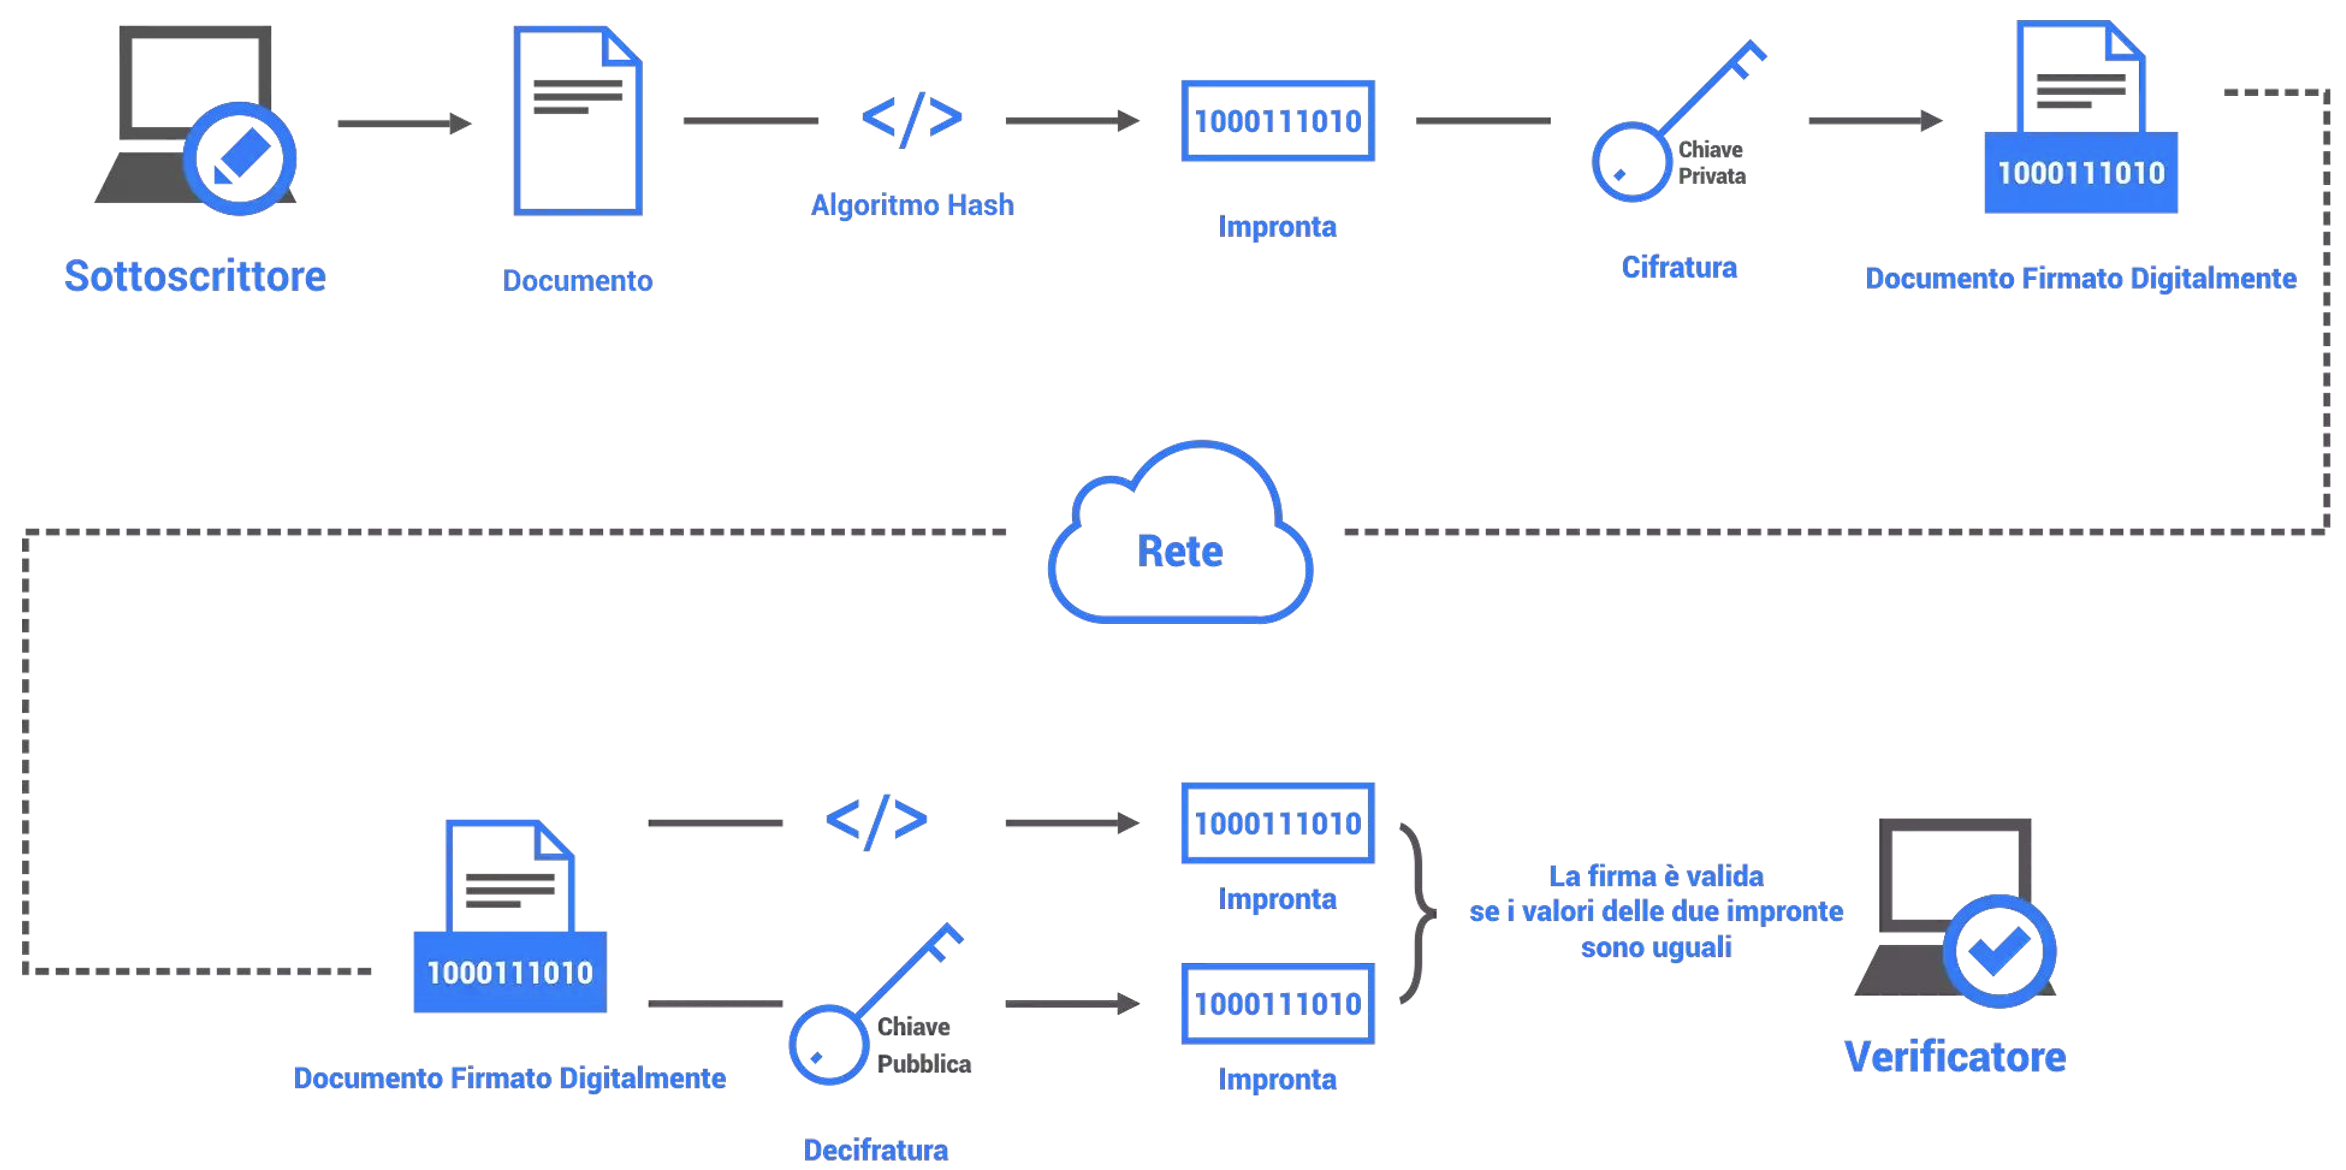
\includegraphics[width=\textwidth]{images/digital_sign.png}
                \caption{Digital signature schematics.}
                \label{fig:digital_sign}
            \end{center}
        \end{figure}
    \end{itemize}

\end{itemize}

\subsection{What Is a VPN?}

A VPN, or Virtual Private Network, is a technology that creates a secure connection over the internet between your device and a remote server or between two devices.

\subsubsection{Main Functions of a VPN}

\begin{itemize}
    \item \textbf{Security}: Encrypts traffic between your device and the VPN server, ensuring intercepted data cannot be read or interpreted.
    \item \textbf{Privacy}: Hides your real IP address and geographic location, making it difficult for websites and online services to track your activity or location.
    \item \textbf{Access to Geo-Blocked Resources}: Allows you to choose a VPN server, enabling you to bypass geographic restrictions.
    \item \textbf{Public Network Security}: Protects you from potential attacks when connected to public Wi-Fi networks, such as in cafes or airports.
\end{itemize}


\section{Python for Hackers and Web Applications}

\section{BUILD WEEK 1: Network Security design}










And this is a nice \texttt{\$\$...\$\$} display environment:
$$
\Delta v = \int\displaylimits_{t_0}^{t_1} a \, \textrm{d}t
$$
Maecenas ut nisi condimentum nisi iaculis porttitor eu sed metus. Proin faucibus aliquet odio, ac lobortis tortor. Mauris porta molestie tortor blandit pretium. Nulla pulvinar id mauris ut efficitur. Donec posuere tortor a odio pellentesque tincidunt. Nulla mi nunc, accumsan nec lectus ut, euismod vulputate libero.
%
And finally we have the \texttt{align/align*} environment:
\begin{align}
x_f - x_i &= \bar{v}t \nonumber\\
\Rightarrow s &= \bar{v}t
\end{align}
%
\section{Yet another section}
\subsection{And a subsection beneath it}
\lecture[1 hour]{13}{06}{2017}
%
\subsection{And now a subsection}
\subsubsection{With a subsubsection following it}
%
Integer pharetra nulla scelerisque purus luctus iaculis. Mauris pulvinar erat non dui pretium, sed vestibulum sapien condimentum. Nam in urna quis sapien rhoncus placerat vitae sit amet odio. Vivamus finibus euismod nibh vestibulum lobortis.\margintext{These ideas were probably discussed in lecture 1 in a parallel universe.} Integer arcu tortor, vestibulum sit amet iaculis ut, ullamcorper non ante. Pellentesque consectetur nec odio quis placerat. Vestibulum vehicula massa vel euismod blandit.
%
%
\margintext{\protect\vspace{2cm}Table \ref{tab:mori} courtesy of Mori, L.F. `Tables in \LaTeX2$\epsilon$: Packages and Methods'.}
\begin{table}[h]
\centering
\begin{tabular}{clcc}
\toprule
\multicolumn{2}{c}{$D$} & $P_u$ & $\sigma_N$\\
\multicolumn{2}{c}{(in)} & (lbs) & (psi)\\\toprule
\multirow{3}*{5} & test 1 & 285 & 38.00\\\cmidrule(l){2-4}
& test 2 & 287 & 38.27\\\cmidrule(l){2-4}
& test 3 & 230 & 30.67\\\midrule
\multirow{3}*{10} & test 1 & 430 & 28.67\\\cmidrule(l){2-4}
& test 2 & 433 & 28.87\\\cmidrule(l){2-4}
& test 3 & 431 & 28.73\\\bottomrule
\end{tabular}
\caption{A table beautified by the \protect\texttt{booktabs} package.}\label{tab:mori}
\end{table}
%
%
\subsubsection{This subsubsection is all by itself}
%
\vskip7ex
\centering
* * *
%
\end{document}%
